%%% Econ713: Microeconomics II
%%% Spring 2021
%%% Danny Edgel
%%%
% Due on Canvas Friday, February 5th, 11:59pm Central Time
%%%

%%%
%							PREAMBLE
%%%

\documentclass{article}

%%% declare packages
\usepackage{amsmath}
\usepackage{amssymb}
\usepackage{array}
\usepackage{bm}
\usepackage{changepage}
\usepackage{centernot}
\usepackage{graphicx}
\usepackage{multirow}
\usepackage[shortlabels]{enumitem}
\usepackage{fancyhdr}
	\fancyhf{} % sets both header and footer to nothing
	\renewcommand{\headrulewidth}{0pt}
    \rfoot{Edgel, \thepage}
    \pagestyle{fancy}
	
%%% define shortcuts for set notation
\newcommand{\N}{\mathbb{N}}
\newcommand{\Z}{\mathbb{Z}}
\newcommand{\R}{\mathbb{R}}
\newcommand{\Q}{\mathbb{Q}}
\newcommand{\lmt}{\underset{x\rightarrow\infty}{\text{lim }}}
\newcommand{\neglmt}{\underset{x\rightarrow-\infty}{\text{lim }}}
\newcommand{\zerolmt}{\underset{x\rightarrow 0}{\text{lim }}}
\newcommand{\usmax}[1]{\underset{#1}{\text{max }}}
\newcommand{\usmin}[1]{\underset{#1}{\text{min }}}
\newcommand{\intersect}{\bigcap}
\newcommand{\union}{\bigcup}
\newcommand{\olw}{\overline{w}}
\newcommand{\olx}{\overline{x}}
\newcommand{\loge}[1]{\text{log}\left(#1\right)}
\renewcommand{\P}{\mathcal{P}}
\renewcommand{\L}{\mathcal{L}}
\newcommand{\olp}{\overline{p}}
\renewcommand{\exp}[1]{\text{exp}\left\{#1\right\}}
\newcommand{\binv}[1]{b_j^{-1}\left(#1\right)}

\DeclareMathOperator{\E}{\mathbb{E}}% expected value

%%% define column vector command (from Michael Nattinger)
\newcount\colveccount
\newcommand*\colvec[1]{
        \global\colveccount#1
        \begin{pmatrix}
        \colvecnext
}
\def\colvecnext#1{
        #1
        \global\advance\colveccount-1
        \ifnum\colveccount>0
                \\
                \expandafter\colvecnext
        \else
                \end{pmatrix}
        \fi
}

%%% define function for drawing matrix augmentation lines
\newcommand\aug{\fboxsep=-\fboxrule\!\!\!\fbox{\strut}\!\!\!}

\makeatletter
\let\amsmath@bigm\bigm

\renewcommand{\bigm}[1]{%
  \ifcsname fenced@\string#1\endcsname
    \expandafter\@firstoftwo
  \else
    \expandafter\@secondoftwo
  \fi
  {\expandafter\amsmath@bigm\csname fenced@\string#1\endcsname}%
  {\amsmath@bigm#1}%
}


%________________________________________________________________%

\begin{document}

\title{	Homework \#1 }
\author{ 	Danny Edgel 					\\ 
			Econ 713: Microeconomics II		\\
			Spring 2021						\\
		}
\maketitle\thispagestyle{empty}

%\noindent\textit{Collaborated with Sarah Bass, Emily Case, Michael Nattinger, and Alex Von Hafften}

%%%________________________________________________________________%%%

\subsection*{Question 1}
If men propose first, then the Gale-Shapley algorithm (i.e. the Deferred Acceptance Algorithm) will end after one round, with man $i$ proposing to woman $i$ and woman $i$, having no other offers, accepting. Thus, the matching would be (1,1), (2,2), and (3,3). If women propose first, then the DAA would end after one round, with W1 proposing to M3, W2 proposing to M1, and W3 proposing to M2 and, each man, having no other offers, accepting their one proposal. Thus, the DAA does not yield the same outcome regardless of who proposes first.
\medskip \\
After the first and third women's preferences change, the male-optimal matching does not change, since the men's preferences have not changed. However, when women propose first, there are multiple rounds:
\begin{enumerate}
	\item W1 and W2 propose to M1; M1 accepts W1. W3 proposes to M3, who accepts.
	\item W2 proposes to M2, who accepts.
\end{enumerate}
In this case, the male-optimal and male-pessimal allocations are the same. According to Gale-Shapley, this means that there is only one stable pairing.

%%%________________________________________________________________%%%
\pagebreak
\subsection*{Question 2}

\begin{enumerate}[(a)]
	\item If men propose first, then the DAA results in M1 and M2 proposing to W2 and M3 proposing to W3 in the first round, with W2 rejecting M1. In the second round, M1 proposes to W1, who accepts. The woman-pessimal matching, then, is (M1,W1), (M2,W2), (M3,W3). If women propose first, W1 proposes to M2, and W2 and W3 propose to M3 in the first round, and M3 rejects W2. In the second round, W2 proposes to M2, and M2 accepts. W1 then proposes to M1, resulting in the same matching as in the male-proposing scenario. Thus, the woman-optimal and woman-pessimal matchings are the same. Therefore, this matching is the only stable one.
	
	\item If side transfers are possible, then the efficient matching is the one that maximizes total utility. In this market, there are only ${3!=6}$ feasible matchings, so they can be checked manually. Of the six matchings, the one that maximizes total payoffs is (M1,W2), (M2,W1), (M3,W3), with a total payoff of 19.\footnote{The table below displays the total payoffs for each matching.
		\begin{center}
			\begin{tabular}{c|c}
				Matching 				& Total Payoff \\ \hline
				(M1,W1),(M2,W2),(M3,W3)	& 17			\\
				(M1,W1),(M2,W3),(M3,W2)	& 12			\\
				(M1,W2),(M2,W1),(M3,W3)	& 19			\\
				(M1,W2),(M2,W3),(M3,W1)	& 13			\\
				(M1,W3),(M2,W1),(M3,W2)	& 16			\\
				(M1,W3),(M2,W2),(M3,W1)	& 15			
			\end{tabular}
		\end{center}
		}
	
	\item Wages of each person in the market must induce the efficient outcome by encouraging efficient matches while discouraging stable but inefficient ones. Thus, in an efficient matching, ${v_2 + w_2\geq 6}$ to discourage an (M2,W2) matching, and ${v_1 + w_2 \leq 4}$ to encourage an (M1,W2) matching. Since the outside option is a payoff of 0, ${v_i,w_i\geq 0}$ for all $i$. Then,
		\begin{align*}
			v_1 + w_2 	\leq 4	&\Rightarrow 0\leq w_2 \leq 4 - v_1					\\
			v_2 + w_2	\geq 6	&\Rightarrow v_2 \geq 6 - w_2 \geq 2 + v_1 \geq 2	
		\end{align*}
		Thus, the minimum wage for M2 is 2.
\end{enumerate}

%%%________________________________________________________________%%%
\pagebreak
\subsection*{Question 3}
In this matching market, the payoff function for $x$, $f(y|x)$, and the payoff function for $y$, $f(x|y)$ are symmetric, with the following marginal payoff functions:
\begin{align*}
	\frac{\partial f}{\partial x}(x|y)	&= 1 + ay	>	0	\\
	\frac{\partial f}{\partial y}(y|x)	&= 1 + ax	>	0
\end{align*}
Thus, type $x$ wants to match with the highest possible type $y$, and type $y$ wants to match with the highest possible type $x$.
\begin{enumerate}[(a)]
	\item If type $x$ proposes first in the DAA algorithm, then in the first round, each $x$ proposes to 1, who accepts 1. In the second round, each $x$ proposes to ${1-\varepsilon\rightarrow 1^-}$, who accepts ${1-\varepsilon}$, and so on. If type $y$ proposes first, then in the first round, each $y$ proposes to 1, who accepts 1. It should be immediately apparent that this market has a unique stable matching, with the following matching function for type $x$:
		\[
			m(y) = y
		\]
	
	\item In a decentralized market, an industry of matching professionals arises to exploit the gains from paying wages to $x$ and $y$ for matching as directed. Matchers make profit ${f(x,y)-w(x)-w(y)}$, where $f(x,y)$ is the output from the match of $x$ to $y$ and $w(\cdot)$ is the wage function. Recall that the output of a match is ${f(x,y)=x+y+2axy}$. The partner, $y$, of $x$ that maximizes $f(x,y)$ is $1-x$. Then, the profit function becomes:
		\[
			\pi(x,y)|_{y=x} = x+y+2axy - w(x) - w(y) 
		\]
	With the first-order condition for $x$:
		\begin{align*}
			\frac{\partial\pi}{\partial x}\bigm|_{y=x} = 1 + 2ay - w'(x) &= 0	\\
														w'(x) = 1 + 2a(1-x)	
		\end{align*}
	Integrating this FOC over $x$ yields:
		\[
			w(x) = x + 2ax - ax^2 + c\text{, }c\in\R
		\]
	Given free entry of matchmakers, we expect $\pi(x,y)=0$ at this maximum. Thus,
		\begin{align*}
			\pi(x,y)|_{y=1-x} = x+y+2axy - w(x) - w(y)  	&= 0				\\
											w(x) + w(1-x)	&= 1 + 2ax(1-x) 	\\
		x + 2ax - ax^2 + c + 1-x + 2a(1-x) - a(1-x)^2 + c	&= 1 + 2ax(1-x)	 	\\
														c	&= -\frac{a}{2}
		\end{align*}
	Thus, a wage of ${w(x)=x + 2ax - ax^2 -\frac{a}{2}}$ can decentralize the market. Given that ${y=1-x}$ is a maximum for $\pi(x,y)$ and $\pi(x,1-x)$ is cleared only by this wage, no other wage could decentralize this market.
\end{enumerate}


%%%________________________________________________________________%%%

\subsection*{Question 4}
Of the borrowers, student $i=1$ has the lowest willingness to pay, accepting any rate below 3.01\%. Student ${i=29}$ has the highest willingness to pay, accepting any rate below 3.29\%. Of the lenders, student ${i=2}$ is willing to accept the lowest rate, of 3.02\%, and student ${i=30}$ requires the highest rate of 3.30\% in order to lend.
\medskip \\
Thus, no student is willing to lend to student 1 at a rate they are willing to pay, and nobody is willing to borrow from 30 at a rate she is willing to charge. Thus, any rate above 3.02\% and below 3.30\% will lead to some number of transactions. Any interest rate below 3.15\% will lead to a credit shortage (i.e. more students willing to borrow than those willing to lend), and any rate above 3.16\% will lead to a surplus. The figure below displays the inverse supply and demand for credit in this market.
\begin{center}
	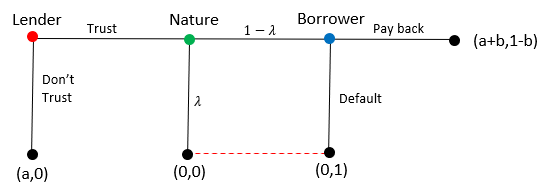
\includegraphics[scale=.5]{figure1.png}
\end{center}



%%%________________________________________________________________%%%


\end{document}
